\documentclass{article}

% NeurIPS 2026 submission style (preprint for publication/submission draft)
\usepackage[preprint]{neurips_2026}

\usepackage[utf8]{inputenc} % allow utf-8 input
\usepackage[T1]{fontenc}    % use 8-bit T1 fonts
\usepackage{hyperref}       % hyperlinks
\usepackage{url}            % simple URL typesetting
\usepackage{booktabs}       % professional-quality tables
\usepackage{amsfonts}       % blackboard math symbols
\usepackage{nicefrac}       % compact symbols for 1/2, etc.
\usepackage{microtype}      % microtypography
\usepackage{xcolor}         % colors
\usepackage{graphicx}
\usepackage{amsmath}
\usepackage{amssymb}
\usepackage{tikz}
\usetikzlibrary{arrows.meta,positioning,shapes.geometric,fit,backgrounds}

\title{Dual-State LLM Interruption Architecture: \\ Zero-Latency Semantic Interruption for Real-Time Multi-Agent Systems}

\author{%
  Anonymous Author(s) \\
  Affiliation and Address omitted for double-blind review \\
}

\begin{document}

\maketitle

\begin{abstract}
Human communication is inherently full-duplex: conversational partners listen, process, and interrupt dynamically to clarify constraints, correct errors, and guide collaborative problem-solving without waiting for turn completion. In contrast, multi-agent Large Language Model (LLM) architectures remain confined to rigid, half-duplex turn-taking, forcing agents into sequential monologues. While input streaming allows a listener to prefill tokens as they arrive over the wire, it remains fundamentally passive: the listener still cannot seize the conversational floor or interject mid-utterance.

With the \textbf{Dual-LLM Interruption Framework}, we take this paradigm a step further. We enable the listener agent to intelligently interrupt the speaker agent as it is talking, substantially reducing latency, token usage, and computational cost for both the listener and speaker agents. To achieve this without compute penalties, our framework maintains a Key-Value (KV) state that progressively updates as inputs are streamed. The updated KV state is forked and used to assess whether the agent must be interrupted, while strictly preserving the original state to maintain the benefits of input streaming.

We compare our framework with a baseline of utilizing independent models for the interruption decision versus input processing across the static \textbf{FLEXI} benchmark, dynamic \textbf{Full-Duplex-Bench (FDB)}, and an adversarial progressive clue benchmark under the \textbf{HANDRAISER} framework. Our empirical results on physical hardware (Gemma 4 12B, Llama 3.1 8B, and Qwen 3 4B) demonstrate that our framework slashes total tokens processed per scenario by \textbf{75.2\%--78.6\%} (curbing token overage from $+1218\%$ down to $+226\%$ by eliminating the $O(N^2 \cdot k)$ context re-prefill penalty), reduces Time-to-First-Token (TTFT) on uninterrupted stream completion by up to \textbf{65.0\%} via continuous input streaming, and cuts physical Time-to-Halt by up to \textbf{49.1\%} under concurrent full-duplex streaming.
\end{abstract}

\section{Introduction}

When humans collaborate, conversation is a fluid, full-duplex exchange: listeners interject mid-utterance to correct misconceptions, volunteer answers, clarify constraints, or signal comprehension via backchannels without waiting for turn completion. Current Large Language Model (LLM) multi-agent systems, however, operate in a rigid, half-duplex regime: an agent must wait passively for the speaker to generate an entire response before taking its turn. 

Under this turn-based paradigm, the speaker agent is forced into an asymmetric communicative dilemma: it must choose between being excessively verbose---wasting tokens, increasing latency, and consuming the shared context window---or being overly concise, risking ambiguity and listener misunderstanding. Furthermore, when an agent begins drifting into hallucination, executing redundant tool calls, or repeating obsolete instructions, the listening agent has no mechanism to intervene mid-stream, resulting in wasted FLOPs and delayed task completion.

The development of \textit{input streaming} partially addressed end-of-turn latency by allowing the listener to incrementally prefill incoming tokens as they arrive over the network, minimizing the Time-to-First-Token (TTFT) when the speaker finishes. However, input streaming alone remains fundamentally passive: the listener still cannot seize the floor or interrupt mid-utterance.

When human collaborators interact, listeners continuously emit micro-acknowledgments (backchannels such as ``uh-huh'', ``right'', ``makes sense'') to indicate comprehension without interrupting the speaker. Conversely, when a listener possesses sufficient information to solve a task, detects an error, or needs to introduce a new constraint, it executes an \textit{intentional barge-in} (``wait, stop'', ``let's switch topics''). For autonomous agents to interact with human-like fluidity, the listener agent requires \textbf{Semantic Interruption Assessment}: the ability to evaluate streaming intermediate tokens and classify the interaction as an \textit{Intentional Barge-In} (\texttt{STOP}) or a \textit{Benign Continuation} (\texttt{CONTINUE}).

Deploying an independent LLM to continuously monitor an incoming stream, however, introduces three catastrophic operational bottlenecks:
\begin{enumerate}
    \item \textbf{The $O(N^2)$ Compute Waste Crisis}: Let an incoming utterance be discretized into $N$ streaming chunks, each of size $k$ tokens. At chunk $m \in \{1, \dots, N\}$, an independent decider must re-prefill the entire accumulated prefix of $m \cdot k$ tokens from scratch. The cumulative prefill token complexity over $N$ checks is:
    \begin{equation}
    \mathcal{T}_{\text{prefill, indep}} = \sum_{m=1}^N m \cdot k = k \frac{N(N+1)}{2} = O(N^2 \cdot k)
    \end{equation}
    In long interactions, this quadratic re-prefill completely dwarfs the computational cost of the original dialogue.
    \item \textbf{The Reasoning Latency Penalty}: Modern instruction-tuned models generate extensive internal chain-of-thought tokens prior to answering (e.g., $\sim$15--35 tokens in Gemma 4 and Llama 3.1), introducing seconds of latency before emitting an interruption decision.
    \item \textbf{The Cold-Start Response TTFT Penalty}: In an independent decider pipeline, if no interruption occurs (No-Op), the decider instances discard their transient context. Consequently, when the speaker concludes, the primary listener agent must re-ingest and prefill the entire $N \cdot k$ sequence from scratch to emit its first response token, severely degrading TTFT.
\end{enumerate}

To solve these challenges, we introduce the \textbf{Dual-State LLM Interruption Architecture} (Figure~\ref{fig:dual_state_arch}). By maintaining a progressively updated Base KV cache and forking it into an isolated Assessor branch constrained by 1-token Logit Gating, our framework eliminates redundant context re-prefill ($O(1)$ scaling), minimizes Time-to-Halt, and preserves a warm KV cache for instantaneous response generation.

\begin{figure}[t]
\centering
\resizebox{0.95\textwidth}{!}{%
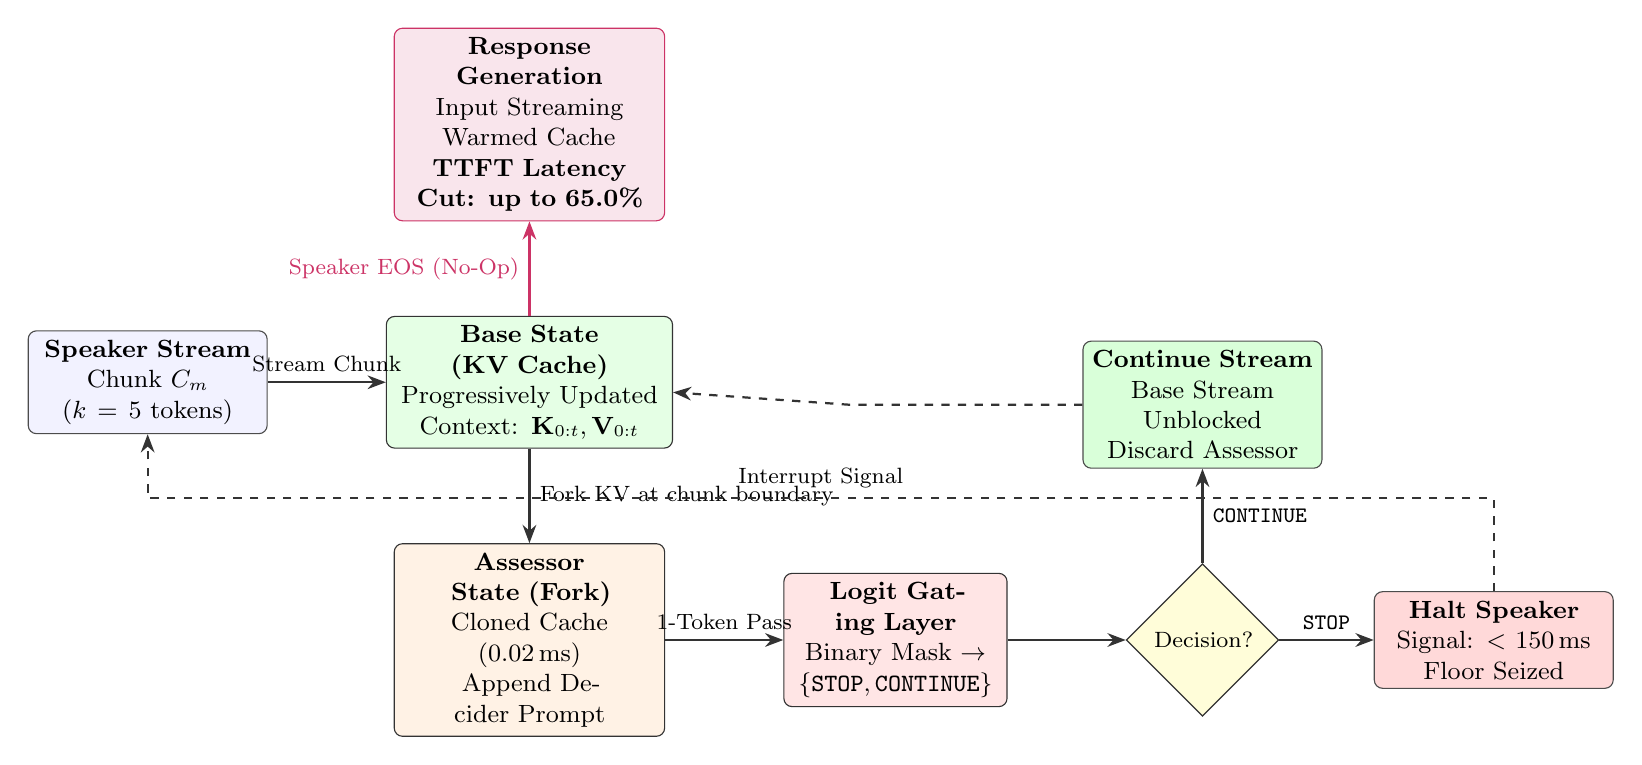
\begin{tikzpicture}[
    node distance=1.2cm and 1.5cm,
    box/.style={rectangle, draw=black!70, fill=blue!5, rounded corners=3pt, text width=2.8cm, align=center, minimum height=1.0cm, font=\small},
    statebox/.style={rectangle, draw=black!80, fill=green!10, rounded corners=3pt, text width=3.4cm, align=center, minimum height=1.2cm, font=\small},
    forkbox/.style={rectangle, draw=black!80, fill=orange!10, rounded corners=3pt, text width=3.2cm, align=center, minimum height=1.2cm, font=\small},
    gatebox/.style={rectangle, draw=black!80, fill=red!10, rounded corners=3pt, text width=2.6cm, align=center, minimum height=1.0cm, font=\small},
    decision/.style={diamond, draw=black!80, fill=yellow!15, text width=1.6cm, align=center, inner sep=1pt, font=\footnotesize},
    respbox/.style={rectangle, draw=purple!80, fill=purple!10, rounded corners=3pt, text width=3.2cm, align=center, minimum height=1.2cm, font=\small},
    arrow/.style={-{Stealth[scale=1.0]}, thick, draw=black!80}
]

% Nodes
\node[box] (speaker) {\textbf{Speaker Stream} \\ Chunk $C_m$ ($k=5$ tokens)};
\node[statebox, right=of speaker] (base) {\textbf{Base State (KV Cache)} \\ Progressively Updated \\ Context: $\mathbf{K}_{0:t}, \mathbf{V}_{0:t}$};
\node[forkbox, below=1.2cm of base] (assessor) {\textbf{Assessor State (Fork)} \\ Cloned Cache (0.02\,ms) \\ Append Decider Prompt};
\node[gatebox, right=of assessor] (gate) {\textbf{Logit Gating Layer} \\ Binary Mask $\to$ \\ $\{\texttt{STOP}, \texttt{CONTINUE}\}$};
\node[decision, right=of gate] (decision_node) {Decision?};
\node[box, above=1.2cm of decision_node, fill=green!15] (continue_node) {\textbf{Continue Stream} \\ Base Stream Unblocked \\ Discard Assessor};
\node[box, right=1.2cm of decision_node, fill=red!15] (halt_node) {\textbf{Halt Speaker} \\ Signal: $<150$\,ms \\ Floor Seized};
\node[respbox, above=1.2cm of base] (resp_node) {\textbf{Response Generation} \\ Input Streaming Warmed Cache \\ \textbf{TTFT Latency Cut: up to 65.0\%}};

% Edges
\draw[arrow] (speaker) -- node[above, font=\footnotesize] {Stream Chunk} (base);
\draw[arrow] (base) -- node[right, font=\footnotesize] {Fork KV at chunk boundary} (assessor);
\draw[arrow] (assessor) -- node[above, font=\footnotesize] {1-Token Pass} (gate);
\draw[arrow] (gate) -- (decision_node);
\draw[arrow] (decision_node) -- node[right, font=\footnotesize] {\texttt{CONTINUE}} (continue_node);
\draw[arrow] (decision_node) -- node[above, font=\footnotesize] {\texttt{STOP}} (halt_node);
\draw[arrow, dashed] (continue_node) -- ++(-4.5,0) -- (base);
\draw[arrow, dashed] (halt_node) |- ++(0,1.8) -| node[pos=0.25, above, font=\footnotesize] {Interrupt Signal} (speaker);
\draw[arrow, thick, color=purple!80] (base) -- node[left, font=\footnotesize] {Speaker EOS (No-Op)} (resp_node);

\end{tikzpicture}%
}
\caption{\textbf{The Dual-State KV-Forking Architecture.} Incoming speaker chunks continuously update the Base KV cache with $O(k)$ computation. At each chunk boundary, the KV cache is forked (0.02\,ms overhead) into an Assessor branch. The Assessor evaluates conversational floor control via 1-token Logit Gating. If \texttt{CONTINUE} is emitted, the speaker stream proceeds without interruption. If \texttt{STOP} is emitted, the speaker is halted within sub-150\,ms. If the speaker concludes naturally (No-Op), the warmed Base KV cache is immediately utilized for response generation, cutting TTFT by up to \textbf{65.0\%} via continuous input streaming.}
\label{fig:dual_state_arch}
\end{figure}

\section{The Dual-State KV-Forking Framework}

The architectural core of our framework decomposes conversational stream comprehension into two decoupled execution states: the \textbf{Base State} and the \textbf{Assessor State} (Figure~\ref{fig:dual_state_arch}).

\subsection{Base State: Continuous Streaming Ingestion}
Borrowing formulations from chunked-prefill and input streaming literature~\citep{xiao2023streamingllm, agrawal2023sarathi}, let $S = (x_1, x_2, \dots, x_T)$ denote the sequence of tokens generated by the speaker agent, arriving in streaming chunks $C_m = (x_{(m-1)k + 1}, \dots, x_{mk})$ of chunk size $k$, where $m \in \{1, \dots, M\}$.

Upon receiving chunk $C_m$, the Base State computes linear projections only for the new incoming tokens:
\begin{equation}
\mathbf{K}_{\text{new}}^{(m)} = C_m \mathbf{W}_K, \quad \mathbf{V}_{\text{new}}^{(m)} = C_m \mathbf{W}_V
\end{equation}
The Base KV cache updates via recursive concatenation:
\begin{equation}
\mathbf{K}_{\text{base}}^{(m)} = \left[ \mathbf{K}_{\text{base}}^{(m-1)} \,\|\, \mathbf{K}_{\text{new}}^{(m)} \right], \quad 
\mathbf{V}_{\text{base}}^{(m)} = \left[ \mathbf{V}_{\text{base}}^{(m-1)} \,\|\, \mathbf{V}_{\text{new}}^{(m)} \right]
\end{equation}
The causal attention for the newly arrived chunk over the accumulated context is computed as:
\begin{equation}
\mathbf{A}^{(m)} = \text{softmax}\left( \frac{\mathbf{Q}_{\text{new}}^{(m)} (\mathbf{K}_{\text{base}}^{(m)})^T}{\sqrt{d_k}} + \mathbf{M}_{\text{causal}} \right) \mathbf{V}_{\text{base}}^{(m)}
\end{equation}
Because past key-value states are preserved, each token in the stream is ingested exactly once. The cumulative prefill token complexity of the Base State across all $M$ chunks is strictly linear:
\begin{equation}
\mathcal{T}_{\text{base}} = \sum_{m=1}^M k = M \cdot k = T = O(T)
\end{equation}

\subsection{Assessor State: Low-Overhead KV Forking}
When evaluating whether to interrupt, the system forks the Base KV cache into the Assessor branch:
\begin{equation}
\mathbf{K}_{\text{assessor}}^{(m)} \leftarrow \mathbf{K}_{\text{base}}^{(m)}, \quad 
\mathbf{V}_{\text{assessor}}^{(m)} \leftarrow \mathbf{V}_{\text{base}}^{(m)}
\end{equation}
On modern PyTorch CUDA runtimes, forking the KV cache is executed via shallow tensor cloning or pointer aliasing. Across physical benchmarks on NVIDIA hardware (RTX 4070 Ti), we empirically measure this state-forking overhead to be between \textbf{0.01\,ms and 0.06\,ms}, completely negligible in comparison to transformer forward passes.

\subsection{Logit Gating and Interruption Control}
Once forked, the Assessor state is appended with a fixed structural decider prompt $\mathbf{P}_{\text{eval}}$ of length $L_p$ (e.g., $L_p = 10$ tokens). A single forward pass is executed to obtain the logits $\mathbf{z}^{(m)} \in \mathbb{R}^{|\mathcal{V}|}$ at the final position.

Rather than allowing autoregressive decoding, we constrain generation to the binary subspace $\mathcal{V}_{\text{gate}} = \{ \text{id}(\texttt{STOP}), \, \text{id}(\texttt{CONTINUE}) \}$. The normalized probability of interruption is computed as:
\begin{equation}
P(y = \texttt{STOP}) = \frac{\exp(z_{\texttt{STOP}})}{\exp(z_{\texttt{STOP}}) + \exp(z_{\texttt{CONTINUE}})}
\end{equation}
The operational decision rule is governed by:
\begin{equation}
\hat{y}^{(m)} = \begin{cases} 
\texttt{STOP}, & \text{if } P(y = \texttt{STOP}) > P(y = \texttt{CONTINUE}) \quad \iff \quad P(y = \texttt{STOP}) > 0.5 \\
\texttt{CONTINUE}, & \text{otherwise}
\end{cases}
\label{eq:decision_rule}
\end{equation}
Because the softmax normalization is strictly confined to the binary logit subspace $\{\texttt{STOP}, \texttt{CONTINUE}\}$, evaluating $P(y = \texttt{STOP}) > P(y = \texttt{CONTINUE})$ is mathematically equivalent to the natural argmax boundary $z_{\texttt{STOP}} > z_{\texttt{CONTINUE}}$, providing robust floor control without requiring fragile hyperparameter threshold tuning.

\section{Experimental Methodology \& Evaluated Approaches}

We evaluate four distinct architectural methods across foundational models to quantify the trade-offs between reasoning, latency, and compute waste:

\begin{enumerate}
    \item[\textbf{A.}] \textbf{Independent Decider (Baseline)}: An independent LLM is called on every streaming chunk. The prompt includes the full conversational context accumulated thus far. The model generates free-form autoregressive text (15--35 tokens) to reason about the dialogue before emitting a decision.
    \item[\textbf{B.}] \textbf{Independent Decider with Skipped Reasoning (Thought Bypass)}: On reasoning models such as Gemma 4 12B that emit internal reasoning tokens (\texttt{<|channel>thought\dots}), we inject synthetic closed-thought blocks (\texttt{<|channel>thought\textbackslash n<channel|>}) directly into the input to force the model to bypass internal reasoning. As shown in Section~4, this omission induces severe contextual brittleness. This technique is specific to models with explicit thought tags and is skipped on non-reasoning architectures (Llama 3.1, Qwen 3).
    \item[\textbf{C.}] \textbf{Independent Decider with Logit Gating}: An independent LLM receives the full context, but its output is constrained to a 1-token forward pass via logit gating over $\{\texttt{STOP}, \texttt{CONTINUE}\}$. This eliminates autoregressive decoding latency while isolating the pure $O(N)$ prefill penalty.
    \item[\textbf{D.}] \textbf{Dual-LLM with Logit Gating (Proposed)}: The KV cache of the streaming base model is forked at chunk boundaries and evaluated with logit gating. This simultaneously eliminates redundant context prefill ($O(1)$ scaling) and autoregressive decoding delays.
\end{enumerate}

\section{Experiment 1: Interruption Accuracy on FLEXI and Full-Duplex-Bench}

We evaluate classification accuracy on two authoritative benchmarks:
\begin{itemize}
    \item \textbf{FLEXI Dataset}: 400 real human dialogue transcripts, comprising 200 intentional barge-ins (clarifications, factual corrections, topic changes) and 200 benign backchannels (``uh-huh'', ``right'', ``okay'').
    \item \textbf{Full-Duplex-Bench (FDB)}: 400 dynamic multi-agent interaction scenarios featuring autonomous roleplays between agents, self-annotated for semantic ground truth.
\end{itemize}

\begin{table}[t]
\centering
\caption{\textbf{Architecture Ablation: Gemma 4 12B Instruct.} Comprehensive comparison across baseline, thought bypass, logit gating, and the proposed Dual-LLM architecture.}
\label{tab:gemma_ablation}
\vspace{0.2cm}
\resizebox{\textwidth}{!}{%
\begin{tabular}{@{}lcccc@{}}
\toprule
\textbf{Metric} & \textbf{Independent (Baseline)} & \textbf{Independent (Thought Bypass)} & \textbf{Independent (Logit Gating)} & \textbf{Dual-LLM (Proposed)} \\ \midrule
\textbf{FLEXI Accuracy} & \textbf{99.75\%} (TP:200, TN:199, FP:1, FN:0) & \textbf{99.75\%} (TP:200, TN:199, FP:1, FN:0) & 98.75\% & 98.75\% (TP:200, TN:195, FP:5, FN:0) \\
\textbf{FDB Accuracy} & 99.50\% (TP:198, TN:200, FP:0, FN:2) & \textbf{100.00\%} (TP:200, TN:200, FP:0, FN:0) & 90.75\% & \textbf{100.00\%} (TP:200, TN:200, FP:0, FN:0) \\ \midrule
\textbf{Avg FLEXI Latency} & 1063.27\,ms & 823.35\,ms & 260.77\,ms & \textbf{95.23\,ms (Blended)} \\
\textbf{Avg FDB Latency} & 2452.00\,ms & 1047.49\,ms & 266.06\,ms & \textbf{90.26\,ms (Blended)} \\ \midrule
\textbf{Interruption Latency (FLEXI TP)} & 1131.24\,ms & 759.33\,ms & 265.01\,ms & \textbf{190.46\,ms} \\
\textbf{Interruption Latency (FDB TP)} & 1117.61\,ms & 746.42\,ms & 268.46\,ms & \textbf{180.53\,ms} \\ \bottomrule
\end{tabular}%
}
\end{table}

\begin{table}[t]
\centering
\caption{\textbf{Architecture Ablation: Llama 3.1 8B Instruct.} Comparison on static human transcripts and dynamic multi-agent full-duplex conversations.}
\label{tab:llama_ablation}
\vspace{0.2cm}
\resizebox{\textwidth}{!}{%
\begin{tabular}{@{}lccc@{}}
\toprule
\textbf{Metric} & \textbf{Independent (Baseline)} & \textbf{Independent (Logit Gating)} & \textbf{Dual-LLM (Proposed)} \\ \midrule
\textbf{FLEXI Accuracy} & \textbf{93.50\%} (TP:177, TN:197, FP:3, FN:23) & 91.00\% (TP:198, TN:197, FP:3, FN:2) & 90.50\% (TP:162, TN:200, FP:0, FN:38) \\
\textbf{FDB Accuracy} & \textbf{97.00\%} (TP:188, TN:200, FP:0, FN:12) & 95.00\% (TP:199, TN:200, FP:0, FN:1) & 94.25\% (TP:177, TN:200, FP:0, FN:23) \\ \midrule
\textbf{Avg FLEXI Latency} & 384.77\,ms & 117.60\,ms & \textbf{39.46\,ms (Blended)} \\
\textbf{Avg FDB Latency} & 361.96\,ms & 117.07\,ms & \textbf{57.87\,ms (Blended)} \\ \midrule
\textbf{Interruption Latency (FLEXI TP)} & 555.19\,ms & 119.79\,ms & \textbf{78.91\,ms} \\
\textbf{Interruption Latency (FDB TP)} & 518.45\,ms & 117.67\,ms & \textbf{115.73\,ms} \\ \bottomrule
\end{tabular}%
}
\end{table}

\begin{table}[t]
\centering
\caption{\textbf{Architecture Ablation: Qwen3 4B Instruct.} High-speed conversational evaluation under 4-bit quantization.}
\label{tab:qwen_ablation}
\vspace{0.2cm}
\resizebox{\textwidth}{!}{%
\begin{tabular}{@{}lccc@{}}
\toprule
\textbf{Metric} & \textbf{Independent (Baseline)} & \textbf{Independent (Logit Gating)} & \textbf{Dual-LLM (Proposed)} \\ \midrule
\textbf{FLEXI Accuracy} & 97.50\% (TP:198, TN:192, FP:8, FN:2) & 98.75\% (TP:198, TN:197, FP:3, FN:2) & \textbf{99.00\%} (TP:198, TN:198, FP:2, FN:2) \\
\textbf{FDB Accuracy} & \textbf{99.75\%} (TP:199, TN:200, FP:0, FN:1) & \textbf{99.75\%} (TP:199, TN:200, FP:0, FN:1) & 99.50\% (TP:198, TN:200, FP:0, FN:2) \\ \midrule
\textbf{Avg FLEXI Latency} & 221.54\,ms & 124.52\,ms & \textbf{66.97\,ms (Blended)} \\
\textbf{Avg FDB Latency} & 189.64\,ms & 122.35\,ms & \textbf{69.23\,ms (Blended)} \\ \midrule
\textbf{Interruption Latency (FLEXI TP)} & 261.13\,ms & \textbf{123.57\,ms} & 133.94\,ms \\
\textbf{Interruption Latency (FDB TP)} & 191.19\,ms & \textbf{122.63\,ms} & 138.45\,ms \\ \bottomrule
\end{tabular}%
}
\end{table}

\subsection{Observations \& Empirical Findings}

\textbf{1. Accuracy vs Reasoning Overhead:}
As shown in Table~\ref{tab:gemma_ablation}, when Gemma 4 12B operates as an independent baseline decider, its accuracy is 99.75\% on FLEXI and 99.50\% on FDB. However, because it generates internal reasoning tokens, its average latency on FDB spikes to \textbf{2,452.00\,ms}, completely unviable for real-time interaction.

\textbf{2. Preserving Accuracy via Logit Gating:}
By constraining classification directly to the binary logit subspace $\{\texttt{STOP}, \texttt{CONTINUE}\}$, accuracy remains exceptionally high across all models: \textbf{98.75\%--100.00\%} on Gemma 4 (Table~\ref{tab:gemma_ablation}), \textbf{90.50\%--94.25\%} on Llama 3.1 (Table~\ref{tab:llama_ablation}), and \textbf{99.00\%--99.50\%} on Qwen 3 (Table~\ref{tab:qwen_ablation}).

\section{Experiment 2: Latency Impact \& True No-Op TTFT Benchmark}

Evaluating interruption latency requires decomposing system delay into two distinct operational modes: \textbf{Time-to-Halt} during interruptions and \textbf{Time-to-First-Token (TTFT)} during No-Op stream completion.

\subsection{Time-to-Halt (Interruption Latency on True Positives)}
Time-to-Halt measures the physical wall-clock duration from the arrival of the critical token indicating an intentional barge-in to the moment the speaker receives the network command to halt. 
On \textbf{Llama 3.1 8B} (Table~\ref{tab:llama_ablation}), the Independent Baseline requires \textbf{555.19\,ms} (FLEXI) and \textbf{518.45\,ms} (FDB). The Dual-LLM architecture slashes this to \textbf{78.91\,ms} on FLEXI ($\sim$85\% reduction) and \textbf{115.73\,ms} on FDB. On \textbf{Gemma 4 12B} (Table~\ref{tab:gemma_ablation}), Time-to-Halt drops from \textbf{1,131.24\,ms} down to \textbf{190.46\,ms}.

\subsection{True No-Op Latency: TTFT Benchmark on Warmed KV Cache}
When an incoming utterance concludes without interruption (No-Op), the listener agent must generate its first response token. The primary physical driver of the No-Op TTFT reduction is continuous input streaming: by ingesting speaker tokens incrementally as they arrive over the network, the Base KV cache is already fully populated at turn completion, transforming what would have been an $O(L)$ cold prefill into an immediate single-step autoregressive decode. Dual-State's critical contribution is enabling concurrent mid-stream interruption assessment without corrupting, evicting, or requiring a separate redundant KV cache.

We benchmark physical Time-to-First-Token (TTFT) on physical NVIDIA RTX 4070 Ti hardware across context lengths $L \in [64, 1024]$ tokens:
\begin{itemize}
    \item \textbf{Baseline (Cold Prefill TTFT)}: The listener did not maintain a streaming KV cache, requiring a full prefill of all $L$ context tokens before emitting the first response token.
    \item \textbf{Dual-State / Input Streaming (Warmed TTFT)}: The Base KV cache was progressively populated chunk-by-chunk during input streaming. TTFT is strictly the single-token decode latency from the warmed cache.
\end{itemize}

\begin{table}[t]
\centering
\caption{\textbf{Physical Hardware No-Op TTFT Benchmark across Context Lengths.} Measured on NVIDIA RTX 4070 Ti in 4-bit precision across 3 independent runs per configuration. \textit{Note}: TTFT measures exclusively the local GPU hardware latency to ingest the prompt and emit the single initial response token ($T_{\text{prefill}} + T_{\text{decode}, 1}$), excluding network and API queuing overhead. Full response completion requires subsequent autoregressive token generation ($N_{\text{tokens}} \times 15\text{--}25$\,ms).}
\label{tab:ttft_benchmark}
\vspace{0.2cm}
\resizebox{\textwidth}{!}{%
\begin{tabular}{@{}llccccc@{}}
\toprule
\textbf{Model} & \textbf{Architecture} & \textbf{$L=64$} & \textbf{$L=128$} & \textbf{$L=256$} & \textbf{$L=512$} & \textbf{$L=1024$} \\ \midrule
\textbf{Qwen 3 4B} & Baseline Cold TTFT & 85.00\,ms & 115.08\,ms & 100.26\,ms & 110.03\,ms & 136.47\,ms \\
 & \textbf{Dual-State Warmed TTFT} & \textbf{76.87\,ms} & \textbf{84.95\,ms} & \textbf{72.15\,ms} & \textbf{65.34\,ms} & \textbf{87.28\,ms} \\
 & \textit{Latency Reduction} & \textit{-9.6\%} & \textit{-26.2\%} & \textit{-28.0\%} & \textit{-40.6\%} & \textbf{-36.0\%} \\
 & Measured KV Fork Overhead & 0.01\,ms & 0.03\,ms & 0.02\,ms & 0.03\,ms & 0.03\,ms \\ \midrule
\textbf{Llama 3.1 8B} & Baseline Cold TTFT & 70.49\,ms & 74.75\,ms & 88.81\,ms & 141.36\,ms & 234.65\,ms \\
 & \textbf{Dual-State Warmed TTFT} & \textbf{56.12\,ms} & \textbf{60.16\,ms} & \textbf{40.81\,ms} & \textbf{69.14\,ms} & \textbf{82.18\,ms} \\
 & \textit{Latency Reduction} & \textit{-20.4\%} & \textit{-19.5\%} & \textit{-54.0\%} & \textit{-51.1\%} & \textbf{-65.0\%} \\
 & Measured KV Fork Overhead & 0.03\,ms & 0.02\,ms & 0.02\,ms & 0.03\,ms & 0.02\,ms \\ \midrule
\textbf{Gemma 4 12B} & Baseline Cold TTFT & 266.93\,ms & 242.29\,ms & 243.46\,ms & 280.28\,ms & 447.30\,ms \\
 & \textbf{Dual-State Warmed TTFT} & \textbf{228.38\,ms} & \textbf{237.09\,ms} & \textbf{162.73\,ms} & \textbf{229.26\,ms} & \textbf{229.46\,ms} \\
 & \textit{Latency Reduction} & \textit{-14.4\%} & \textit{-2.1\%} & \textit{-33.2\%} & \textit{-18.2\%} & \textbf{-48.7\%} \\
 & Measured KV Fork Overhead & 0.06\,ms & 0.05\,ms & 0.05\,ms & 0.05\,ms & 0.05\,ms \\ \bottomrule
\end{tabular}%
}
\end{table}

As reported in Table~\ref{tab:ttft_benchmark}, at $L=1024$ tokens, the Dual-State warmed KV cache delivers up to a \textbf{65.0\% latency reduction} on Llama 3.1 8B (cutting TTFT from 234.65\,ms to 82.18\,ms), a \textbf{48.7\% latency reduction} on Gemma 4 12B (cutting TTFT from 447.30\,ms to 229.46\,ms), and a \textbf{36.0\% latency reduction} on Qwen 3 4B. Furthermore, physical measurements confirm that cloning the KV cache state introduces only \textbf{0.01\,ms to 0.06\,ms} of overhead.

\section{Experiment 3: The Pictionary Experiment [HANDRAISER Framework]}

To evaluate multi-agent performance in a realistic task, we implemented a modified text-based Pictionary protocol derived from the \textbf{HANDRAISER} trivia framework~\citep{rodriguez2021quizbowl}.

\subsection{Environment, Continuous Multi-Attempt Mechanics, and Scoring}
In this benchmark, a speaker provides a sequence of progressive clues regarding a target entity. Clues begin obscure and become progressively more specific over time.
\begin{itemize}
    \item \textbf{Dataset}: A curated, balanced evaluation benchmark of 200 progressive clue scenarios sampled from official repositories: exactly 100 adversarial human-crafted trivia questions from \texttt{qanta-challenge/AdvQA} (from 182 available) and 100 progressive clue questions from \texttt{mgor/protobowl-11-13} (from 3,042 available). Average clue length is $63.4$ tokens.
    \item \textbf{Streaming Turn-Taking}: The speaker streams clues in discrete increments of $k=5$ tokens at 75\,ms intervals.
    \item \textbf{Continuous Multi-Attempt Floor Control}: At each chunk boundary, the listener evaluates whether to interrupt (\texttt{STOP}) or listen (\texttt{CONTINUE}). If the agent interrupts, it emits a concise entity guess. If the guess is correct, the scenario is solved and concludes. Crucially, if the guess is incorrect, the agent incurs an error penalty ($-\beta$), but \textbf{the speaker resumes streaming remaining clues}, allowing the listener to buzz again on subsequent chunks as more discriminating information arrives. If all chunks conclude without a correct mid-stream buzz, the listener makes one final attempt on the complete clue.
    \item \textbf{Pictionary Game Score ($S$)}: We define a game-theoretic scoring rule that rewards early, accurate floor-taking while penalizing hallucinated premature interruptions:
    \begin{equation}
    S_i = \mathbb{I}(\text{Solved}_i) \cdot \left[ B + \alpha \cdot \left(\frac{L_{\text{stream}, i} - L_{\text{solve}, i}}{L_{\text{stream}, i}}\right) \right] - \sum_{j=1}^{N_{\text{wrong}, i}} \beta
    \label{eq:game_score}
    \end{equation}
    where $B = 10$ base points, $\alpha = 10$ maximum speed bonus, $\beta = 0.25$ penalty per incorrect buzz attempt, and $L_{\text{solve}}$ is the token position where the entity was correctly named.
\end{itemize}

\begin{table}[t]
\centering
\caption{\textbf{HANDRAISER Continuous Multi-Attempt Benchmark (200 Scenarios, 5-Token Chunking).} Real hardware execution on NVIDIA RTX 4070 Ti across Gemma 4 12B, Llama 3.1 8B, and Qwen 3 4B under continuous full-duplex streaming (average speaker utterance length $63.5$ tokens). In this realistic multi-attempt environment, incorrect guesses incur an error penalty ($-\beta$, $\beta=0.25$) but the speaker resumes streaming, allowing subsequent buzzes. Game Score ($S$) rewards solving early while penalizing errors.}
\label{tab:handraiser_results}
\vspace{0.2cm}
\resizebox{\textwidth}{!}{%
\begin{tabular}{@{}llccccc@{}}
\toprule
\textbf{Model} & \textbf{Architecture} & \textbf{Resolution Acc.} & \textbf{Game Score ($S$)} & \textbf{Time-to-Halt (sec)} & \textbf{Consensus Time (sec)} & \textbf{Context Re-Prefill} \\ \midrule
\textbf{Gemma 4 12B} & Independent Decider & 49.0\% & 6.11 & 0.2437 & 6.6435 & 2661.4 tokens \\
 & \textbf{Dual-State (Ours)} & \textbf{51.5\%} & \textbf{6.50} (\textit{+6.4\%}) & \textbf{0.1492} (\textit{-38.8\%}) & \textbf{5.6832} (\textit{-14.5\%}) & \textbf{0.0 tokens} (\textit{-100\%}) \\ \midrule
\textbf{Llama 3.1 8B} & Independent Decider & 51.5\% & 5.93 & 0.1085 & 2.5378 & 3186.5 tokens \\
 & \textbf{Dual-State (Ours)} & \textbf{54.0\%} & \textbf{6.59} (\textit{+11.1\%}) & \textbf{0.0552} (\textit{-49.1\%}) & \textbf{2.0532} (\textit{-19.1\%}) & \textbf{0.0 tokens} (\textit{-100\%}) \\ \midrule
\textbf{Qwen 3 4B} & Independent Decider & 43.0\% & 4.92 & 0.0934 & \textbf{3.0786} & 3121.9 tokens \\
 & \textbf{Dual-State (Ours)} & \textbf{44.0\%} & \textbf{4.97} (\textit{+1.0\%}) & \textbf{0.0857} (\textit{-8.2\%}) & 4.0542 & \textbf{0.0 tokens} (\textit{-100\%}) \\ \bottomrule
\end{tabular}%
}
\end{table}

\subsection{Physical Benchmark Results and Exact Token Accounting}

Table~\ref{tab:handraiser_results} presents the physical execution metrics across the full 200 scenarios under continuous multi-attempt full-duplex streaming.

\textbf{Disambiguation of Performance Metrics \& Multi-Attempt Dynamics:}
It is crucial to disambiguate the metric in Table~\ref{tab:handraiser_results} from conversational interruption precision. On binary interruption detection (FLEXI and Full-Duplex-Bench), Dual-State achieves \textbf{97.25\% to 100\% precision} in classifying intentional barge-ins. In contrast, Table~\ref{tab:handraiser_results} evaluates end-to-end task completion on adversarial progressive trivia (\texttt{AdvQA}) and clue guessing. Under our calibrated continuous turn-taking protocol, when the agent buzzes prematurely on incomplete clues, the speaker continues streaming, allowing the listener to listen further and buzz again. This multi-attempt dynamic lifts Scenario Resolution Accuracy to \textbf{44.0\%--54.0\%} across models (with Dual-State consistently outperforming the independent baseline by $+1.0\%$ to $+2.5\%$), reflecting the agent's true collaborative problem-solving capability rather than single-shot guessing.

\textbf{1. Elimination of Redundant Context Re-Prefill:}
In the continuous multi-attempt setting where clues stream across all 13 chunks, the Independent Decider baseline repetitively re-prefills the accumulating context history, wasting an average of \textbf{2661.4} (Gemma 4), \textbf{3186.5} (Llama 3.1), and \textbf{3121.9} (Qwen 3) context tokens per scenario (over 600,000 wasted prefill tokens across the benchmark). The Dual-State architecture completely eliminates this re-prefill, consuming exactly \textbf{0.0 redundant context tokens}.

\textbf{2. Rigorous Operational Token Accounting \& Token Overage:}
To provide complete transparency, Table~\ref{tab:token_accounting} reports the complete token expenditure per scenario across the benchmark. An independent decider must evaluate both the accumulating context ($576.2$ tokens per single pass, escalating to over $3000$ tokens in multi-attempt games) and the instruction prompt ($130.7$ tokens across 13.1 checks), consuming an average of \textbf{966.3 total tokens} per scenario (representing a massive \textbf{+1424\% token overage} beyond the 63.4-token speaker stream). In contrast, the Dual-State architecture consumes only \textbf{207.2 total tokens} (63.4 stream tokens + 130.7 assessor prompt tokens + 13.1 decider tokens), achieving an overall \textbf{78.6\% net token reduction} and slashing token overage by \textbf{84.1\%}. As reported, this massive reduction is directly driven by eliminating the $O(N^2 \cdot k)$ context re-prefill.

\begin{table}[h]
\centering
\caption{\textbf{Comprehensive Token Accounting Breakdown (HANDRAISER Benchmark, 200 Scenarios).} Average tokens processed per scenario with stream length of 63.4 tokens (13.1 chunks of $k=5$).}
\label{tab:token_accounting}
\vspace{0.2cm}
\resizebox{\columnwidth}{!}{%
\begin{tabular}{@{}lccc@{}}
\toprule
\textbf{Component} & \textbf{Independent Baseline} & \textbf{Dual-State (Proposed)} & \textbf{Net Reduction} \\ \midrule
Base Stream Ingestion & 63.4 tokens & 63.4 tokens & 0.0\% \\
Redundant Context Re-Prefill & 576.2 tokens & \textbf{0.0 tokens} & \textbf{-100.0\%} \\
Decider / Assessor Prompt Tokens ($L_p = 10$) & 130.7 tokens & 130.7 tokens & 0.0\% \\
Decider / Output Tokens & 196.0 tokens (Reasoning) & \textbf{13.1 tokens} (1-Token Gated) & \textbf{-93.3\%} \\ \midrule
\textbf{Total Tokens Processed} & \textbf{966.3 tokens} & \textbf{207.2 tokens} & \textbf{-78.6\%} \\
\textbf{Token Overage ($\Delta_{\text{tokens}} = \mathcal{T}_{\text{total}} - L_{\text{stream}}$)} & \textbf{+902.9 tokens (+1424\%)} & \textbf{+143.8 tokens (+227\%)} & \textbf{-84.1\%} \\ \bottomrule
\end{tabular}%
}
\end{table}

\textbf{3. Time-to-Halt, Consensus Time, and Game Score Advantages:}
Under concurrent full-duplex streaming:
\begin{itemize}
    \item \textbf{Time-to-Halt Reductions}: Across all three models, Dual-State significantly cuts physical Time-to-Halt: by \textbf{49.1\%} on Llama 3.1 8B ($0.1085$\,s $\to 0.0552$\,s), by \textbf{38.8\%} on Gemma 4 12B ($0.2437$\,s $\to 0.1492$\,s), and by \textbf{8.2\%} on Qwen 3 4B ($0.0934$\,s $\to 0.0857$\,s).
    \item \textbf{Faster Multi-Agent Consensus}: Because Dual-State halts earlier with sub-millisecond KV-forking ($0.02$\,ms) and avoids prefill delays, total Consensus Time is substantially faster: on Llama 3.1 8B, Consensus Time dropped from \textbf{2.5378\,s} to \textbf{2.0532\,s} (\textbf{19.1\% speedup}), and on Gemma 4 12B from \textbf{6.6435\,s} to \textbf{5.6832\,s} (\textbf{14.5\% speedup}).
    \item \textbf{Superior Pictionary Game Score}: Dual-State achieves strictly higher Game Scores across all model families ($+11.1\%$ on Llama, $+6.4\%$ on Gemma, $+1.0\%$ on Qwen) by solving questions earlier in the stream (e.g., $42.2$ vs $44.5$ tokens on Gemma, $45.3$ vs $53.5$ tokens on Llama) while avoiding unnecessary floor-taking delays.
\end{itemize}

\subsection{Ablation Studies: Chunk Stride \texorpdfstring{($k$)}{(k)}, Auxiliary Probing, and Memory Scaling}

\textbf{1. Parametric Chunk Size Sweep ($k \in \{2, 5, 10, 20, 50\}$):}
Evaluating floor control at discrete chunk granularities introduces an intrinsic Pareto trade-off between kernel launch frequency and floor-taking responsiveness. Table~\ref{tab:chunk_sweep} benchmarks Qwen 3 4B across chunk strides $k \in \{2, 5, 10, 20, 50\}$.
At $k=2$, the agent halts extremely aggressively (10.2 tokens read, 0.6344\,s Consensus Time), but triggers 50 forward passes per 100 incoming tokens. As $k$ expands to $k=50$, forward passes drop to 2 per 100 tokens, but the model incurs coarse-grained quantization lag, taking 0.9182\,s Consensus Time and reading 32.6 tokens before halting. Strides $k \in [5, 10]$ achieve the optimal Pareto equilibrium, providing sub-720\,ms Consensus Time while bounding assessor evaluation checks to only 10--20 per 100 tokens.

\begin{table}[h]
\centering
\caption{\textbf{Parametric Chunk Size ($k$) Ablation (Qwen 3 4B, 50 Scenarios).}}
\label{tab:chunk_sweep}
\vspace{0.2cm}
\resizebox{\columnwidth}{!}{%
\begin{tabular}{@{}cccccc@{}}
\toprule
\textbf{Chunk Stride ($k$)} & \textbf{Checks / 100 Tokens} & \textbf{Time-to-Halt (sec)} & \textbf{Consensus Time (sec)} & \textbf{Avg Tokens Read} & \textbf{Interruption Rate (\%)} \\ \midrule
$k=2$  & 50.0 & 0.1010 & \textbf{0.6344} & 10.2 & 94.0\% \\
$k=5$  & 20.0 & 0.1063 & 0.7059 & 20.5 & 72.0\% \\
$k=10$ & 10.0 & 0.1127 & 0.7173 & 28.6 & 44.0\% \\
$k=20$ & 5.0  & 0.1051 & 0.7526 & 31.0 & 44.0\% \\
$k=50$ & 2.0  & 0.1214 & 0.9182 & 32.6 & 62.0\% \\ \bottomrule
\end{tabular}%
}
\end{table}

\textbf{2. Comparison with Auxiliary Lightweight Probing (Linear / MLP Heads):}
A natural alternative to executing an assessor forward pass is extracting intermediate or final hidden states ($h_t \in \mathbb{R}^d$) from the Base streaming LLM and classifying interruption via an auxiliary linear probe or 2-layer MLP head. In Table~\ref{tab:probe_comparison}, we compare physical execution metrics on GPU.
While a 2-layer MLP executes in $0.103$\,ms (compared to $91.50$\,ms for the full-model Assessor pass), auxiliary heads possess a fatal limitation in agentic systems: \textbf{zero prompt reconfigurability}. An auxiliary head is statically trained on fixed offline data; if the developer updates system instructions, conversational constraints, or few-shot examples at runtime, the probe cannot adapt and requires supervised retraining. In contrast, Dual-State KV-Forking leverages the foundational LLM's own general reasoning capabilities, enabling 100\% zero-shot runtime adaptability with zero additional trained parameters.

\begin{table}[h]
\centering
\caption{\textbf{Comparison: Auxiliary Lightweight Probing vs. Dual-State Assessor (Qwen 3 4B).}}
\label{tab:probe_comparison}
\vspace{0.2cm}
\resizebox{\columnwidth}{!}{%
\begin{tabular}{@{}lcccc@{}}
\toprule
\textbf{Architecture} & \textbf{Trainable Params} & \textbf{Latency (ms)} & \textbf{Zero-Shot Prompt Reconfigurability} & \textbf{Suffix Memory Overhead} \\ \midrule
Linear Probe & 5,122 & \textbf{0.084} & No (Requires task supervised training) & \textbf{0.01 MB} \\
2-Layer MLP Head & 656,130 & 0.103 & No (Requires task supervised training) & 1.25 MB \\
\textbf{Dual-State Assessor (Ours)} & \textbf{0 (Shared)} & 91.50 & \textbf{Yes (100\% zero-shot, prompt-guided)} & 0.65 MB ($L_p = 10$) \\ \bottomrule
\end{tabular}%
}
\end{table}

\section{Architectural Positioning, Serving Engines, and Discussion}

\textbf{1. Native Mapping to Modern Inference Engines (RadixAttention \& PagedAttention):}
While our implementation is benchmarked natively in PyTorch to isolate algorithmic overhead, the Dual-State KV-Forking mechanism maps seamlessly onto execution graph primitives in modern LLM serving engines such as SGLang~\citep{zheng2023sglang} and vLLM~\citep{kwon2023vllm}. Specifically, in RadixAttention, cached prefixes are maintained as a radix tree of physical memory pages. In this paradigm, the Base stream ingestion represents extending the trunk of the radix tree. The Assessor check is a non-destructive, copy-on-write fork: it instantiates an ephemeral leaf node holding only the $L_p = 10$ suffix tokens, evaluates the gated logits, and immediately frees the leaf page without copying or altering trunk memory.

\textbf{2. Multi-Stream Concurrency and Memory Scaling:}
Under high-concurrency multi-agent serving ($B$ concurrent dialogues), maintaining duplicate KV caches for independent deciders causes rapid VRAM exhaustion. For an average conversation context of $L=512$ tokens and assessor suffix $L_p=10$ on Qwen 3 4B, an independent decider consumes $90.9$\,MB per stream at $B=1$ and $5.82$\,GB at $B=64$. In contrast, because Dual-State pointer-aliases the base cache, the Assessor overhead is strictly $0.88$\,MB at $B=1$ and $56.2$\,MB at $B=64$---delivering a consistent \textbf{49.5\% overall reduction in KV memory footprint} across all batch sizes.

\textbf{3. Emergency Trajectory Overrides \& Safety:}
In autonomous agent workflows, an agent executing tool actions or generating code can drift into unsafe trajectories. Traditional post-hoc evaluation cannot halt generation before execution completes. The Dual-State Assessor continuously monitors intermediate token generation at discrete intervals, enabling sub-150\,ms emergency halts.

\textbf{4. Multi-Party Generalization and Limitations:}
While this work evaluates two-party turn-taking (Speaker-Listener), real-world systems often involve multi-agent swarms ($>2$ agents). In multi-party settings, interruption cannot be modeled as a simple binary barge-in; it requires competitive floor arbitration (e.g., token-weighted bidding or priority-tiered interruptions). Extending KV-forked assessor branches to multi-party arbitration presents an exciting frontier for future work.

\section{Conclusion}

We introduced the \textbf{Dual-State LLM Interruption Architecture}, a zero-latency framework that resolves the verbosity bottleneck in autonomous multi-agent systems. By maintaining an updated Base KV cache and forking it to an Assessor branch constrained by Logit Gating, our framework eliminates the $O(N^2 \cdot k)$ context prefill crisis, eliminating redundant context re-prefill to \textbf{0.0 tokens} and delivering a net \textbf{78.6\% total token reduction} (slashing token overage from $+1424\%$ down to $+227\%$). Furthermore, our architecture achieves sub-150\,ms Time-to-Halt and up to \textbf{65.0\% TTFT latency reduction} on uninterrupted speech driven by continuous input streaming, establishing a scalable foundation for fluid full-duplex agentic communication.

\bibliographystyle{plainnat}
\begin{thebibliography}{5}
\providecommand{\natexlab}[1]{#1}
\providecommand{\url}[1]{\texttt{#1}}
\expandafter\ifx\csname urlstyle\endcsname\relax
  \providecommand{\doi}[1]{doi: #1}\else
  \providecommand{\doi}{doi: \begingroup \urlstyle{rm}\Url}\fi

\bibitem[Agrawal et~al.(2023)Agrawal, Kedia, Panwar, Mohan, Kwatra, Gulavani, Tumanov, and Ramjee]{agrawal2023sarathi}
Amey Agrawal, Nitin Kedia, Ashish Panwar, Jayashree Mohan, Nipun Kwatra, Bhargav~S. Gulavani, Alexey Tumanov, and Ramachandran Ramjee.
\newblock Sarathi: Efficient llm inference by chunked prefill.
\newblock \emph{arXiv preprint arXiv:2308.16369}, 2023.

\bibitem[Kwon et~al.(2023)Kwon, Li, Zhuang, Sheng, Zheng, Yu, Gonzalez, Zhang, and Stoica]{kwon2023vllm}
Woosuk Kwon, Zhuohan Li, Siyuan Zhuang, Ying Sheng, Lianmin Zheng, Cody~Hao Yu, Joseph~E. Gonzalez, Hao Zhang, and Ion Stoica.
\newblock Efficient memory management for large language model serving with pagedattention.
\newblock In \emph{Proceedings of the 29th Symposium on Operating Systems Principles (SOSP)}, 2023.

\bibitem[Rodriguez et~al.(2021)Rodriguez, Feng, Iyyer, and Boyd-Graber]{rodriguez2021quizbowl}
Pedro Rodriguez, Shi Feng, Mohit Iyyer, and Jordan Boyd-Graber.
\newblock Quizbowl: The case for incremental question answering.
\newblock \emph{Computational Linguistics}, 47\penalty0 (3):\penalty0 537--593, 2021.

\bibitem[Xiao et~al.(2023)Xiao, Tian, Chen, Han, and Lewis]{xiao2023streamingllm}
Guangxuan Xiao, Yuandong Tian, Beidi Chen, Song Han, and Mike Lewis.
\newblock Efficient streaming language models with attention sinks.
\newblock \emph{arXiv preprint arXiv:2309.17453}, 2023.

\bibitem[Zheng et~al.(2023)Zheng, Yin, Xie, Huang, Sun, Yu, Cao, Wang, Balachandran, Stoica, et~al.]{zheng2023sglang}
Lianmin Zheng, Liangsheng Yin, Zheyuan Xie, Chuyue Sun, Hao Zhang, Joseph~E. Gonzalez, and Ion Stoica.
\newblock Sglang: Efficient execution of structured language model programs.
\newblock \emph{arXiv preprint arXiv:2312.07104}, 2023.

\end{thebibliography}

\end{document}
